% Compile to an SVG with:
%
%     pdflatex tixz-learn.tex
%     inkscape tixz-learn.pdf --export-type=svg --export-filename=tixz-learn.svg

\documentclass[crop,tikz]{standalone}
\usepackage{amsmath}

\begin{document}

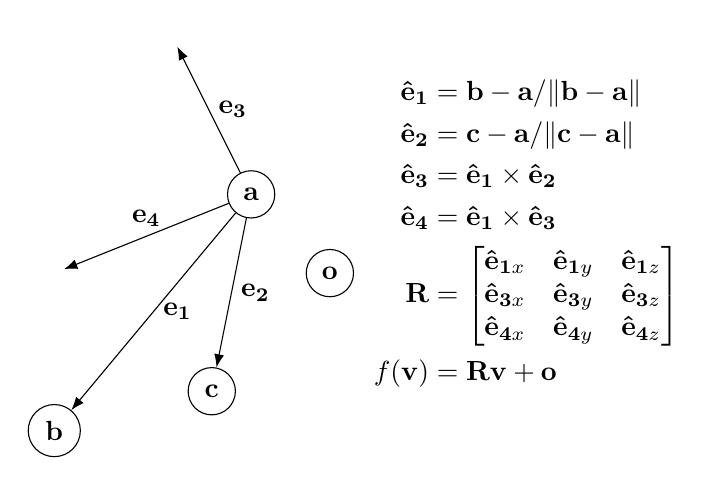
\begin{tikzpicture}[
		trianglenode/.style={
		% The shape:
		circle,
		% The size:
		minimum size=6mm,
		% The border:
		%very thick,
		draw=black,
		% The filling:
		top color=white,
		bottom color=white,
		% Font
		font=\itshape
    		}
	]
	% latex-latexnew, o-onenew, etc. arrows (see: https://tex.stackexchange.com/questions/5461/is-it-possible-to-change-the-size-of-an-arrowhead-in-tikz-pgf)
	\usetikzlibrary{arrows.meta}
	\usetikzlibrary{matrix}
	
	\node (A)[trianglenode] at (3.5,5) {$\mathbf{a}$};
	\node (B)[trianglenode] at (1,2)  {$\mathbf{b}$};
	\node (C)[trianglenode] at (3,2.5) {$\mathbf{c}$};
	\node (E3) at (2.5,7) {};
	\node (E4) at (1,4) {};
	\node (O)[trianglenode] at (4.5, 4) {$\mathbf{o}$};
	
	\node (EQN)[align=left] at (7,4.5) {$
		\begin{aligned}
			\mathbf{\hat{e}_1} &= \mathbf{b - a} / \|\mathbf{b - a}\| \\
			\mathbf{\hat{e}_2} &= \mathbf{c - a} / \|\mathbf{c - a}\| \\
			\mathbf{\hat{e}_3} &= \mathbf{\hat{e}_1 \times \hat{e}_2} \\
			\mathbf{\hat{e}_4} &= \mathbf{\hat{e}_1 \times \hat{e}_3} \\
			\mathbf{R} &= \begin{bmatrix}
			    \mathbf{\hat{e}}_{\mathbf{1}x} & \mathbf{\hat{e}}_{\mathbf{1}y} & \mathbf{\hat{e}}_{\mathbf{1}z} \\
			    \mathbf{\hat{e}}_{\mathbf{3}x} & \mathbf{\hat{e}}_{\mathbf{3}y} & \mathbf{\hat{e}}_{\mathbf{3}z} \\
			    \mathbf{\hat{e}}_{\mathbf{4}x} & \mathbf{\hat{e}}_{\mathbf{4}y} & \mathbf{\hat{e}}_{\mathbf{4}z} \end{bmatrix} \\
			f(\mathbf{v}) &= \mathbf{Rv} + \mathbf{o}
		\end{aligned}
	$};

  	\draw [-Latex] (A) -- node[anchor=west]  {$\mathbf{e_1}$} (B);
  	\draw [-Latex] (A) -- node[anchor=west]  {$\mathbf{e_2}$} (C);
  	\draw [-Latex] (A) -- node[anchor=west]  {$\mathbf{e_3}$} (E3);
  	\draw [-Latex] (A) -- node[anchor=south] {$\mathbf{e_4}$} (E4);
\end{tikzpicture}
\end{document}